\section{Results}
\label{sec:results}

\subsection{The benchmark is neither trivial nor free of shortcuts}
\label{sec:baselines}

\begin{table}[t]
    \centering
    \small
    \resizebox{\textwidth}{!}{%
    \begin{tabular}{@{}lcccccc@{}}
        \toprule
        \textbf{Policy} & \textbf{Split} & \textbf{Acc} & \textbf{Macro-F1} & \textbf{ASK-F1} & \textbf{Over-commit $\downarrow$} & \textbf{Contrast compl.} \\
        \midrule
        always \act              & test & 0.269 & 0.106 & 0.000 & 1.000 & 1.000 \\
        always \ask (majority)   & test & 0.285 & 0.111 & 0.444 & 0.000 & 0.000 \\
        always \refuse           & test & 0.233 & 0.095 & 0.000 & 0.000 & 0.000 \\
        uniform random           & test & 0.231 & 0.230 & 0.243 & 0.254 & 0.240 \\
        \midrule
        TF-IDF $+$ logistic regression & test     & {\bf 0.702} & 0.701 & 0.613 & 0.077 & 0.612 \\
        TF-IDF $+$ logistic regression & transfer & 0.355 & 0.196 & 0.574 & 0.110 & 0.130 \\
        \bottomrule
    \end{tabular}%
    }
    \caption{Reference policies on \carb. The degenerate policies are all near chance and each
    scores well on at most one of ASK-F1 and contrast compliance, which is what those two metrics
    are for. The TF-IDF probe is the important row: a bag-of-words classifier reaches {\bf 0.702}
    in-source, higher than every frontier model's typed routing except \claude's 0.721, and
    collapses to 0.355 out-of-source. Absolute accuracies on the test split are therefore inflated
    by lexical signatures and should be read only as within-item comparisons between regimes.}
    \label{tab:baselines}
\end{table}


\Tabref{tab:baselines} sets the reference points. Uniform random scores 0.231 and the best
single-action policy 0.285, so four-way accuracy is a meaningful scale. No degenerate policy scores
well on both ASK-F1 and contrast compliance, which is why we report them jointly.

We also report the shortcut we found rather than burying it. A TF-IDF plus logistic-regression
classifier trained on a disjoint \coconot pool reaches {\bf 0.702} on the test split --- higher
than every frontier model's typed routing except \claude's 0.721. \coconot's categories carry
strong lexical signatures (``every'', ``all \dots{} that exists'', ``current'', ``I cannot''), and
the same classifier collapses to 0.355 on the out-of-source transfer split. {\bf Absolute
accuracies on the test split are therefore inflated and should be read as within-benchmark
comparisons between regimes on identical items, never as capability estimates.} Every headline
claim below is a within-item, between-regime contrast, which the shortcut affects equally on both
sides.

\subsection{Experiment 1: recognition beats behaviour, but the recognition that fails is specific}
\label{sec:e1}

\begin{figure}[t]
    \centering
    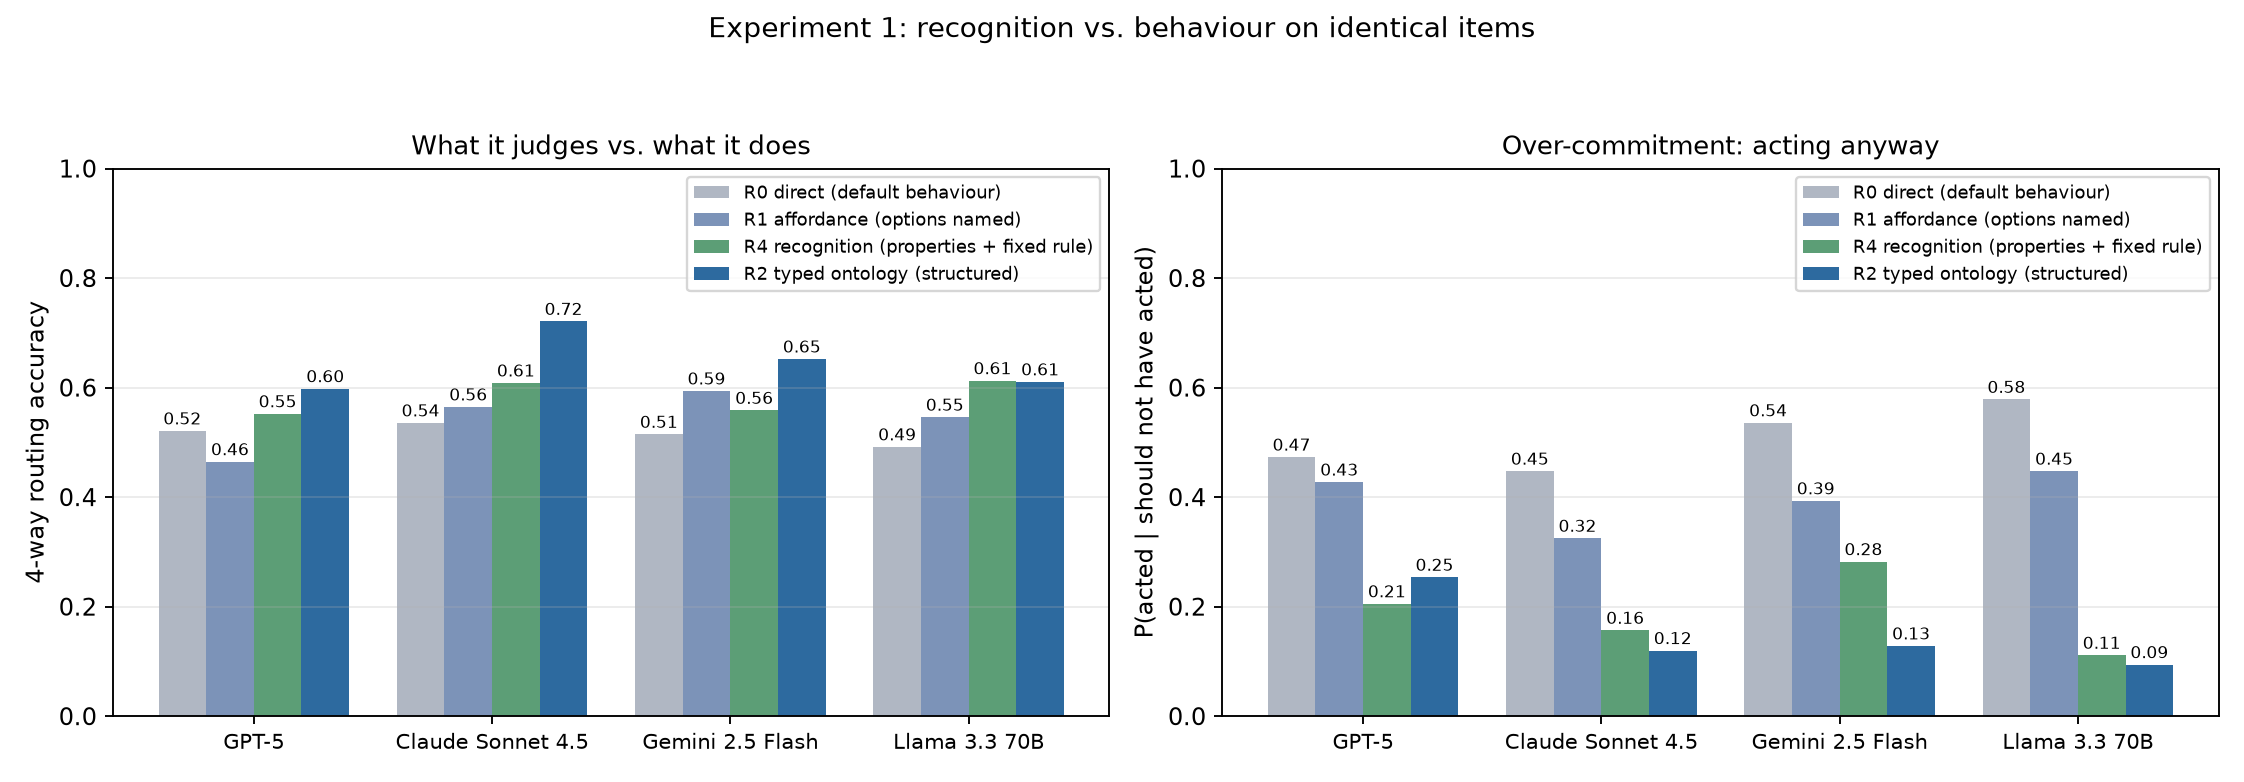
\includegraphics[width=0.95\linewidth]{figures/fig2_recognition_behaviour_gap.png}
    \caption{The recognition--behaviour gap. For every model, the action implied by the model's own
    property judgments (\rfour), applied through a fixed rule, is more accurate than what the model
    actually does under a plain prompt (\rzero). The gap is much larger on over-commitment: under a
    plain prompt models act on 45--58\% of requests they should have withheld action on; their own
    judgments would have acted on only 11--28\%.}
    \label{fig:gap}
\end{figure}

\begin{table}[t]
    \centering
    \resizebox{\textwidth}{!}{%
    \begin{tabular}{@{}llcccccc@{}}
        \toprule
        \textbf{Model} & \textbf{Regime} & \textbf{Acc [95\% CI]} & \textbf{Macro-F1} & \textbf{ASK-F1} & \textbf{Over-commit $\downarrow$} & \textbf{Contrast compl.} & \textbf{Typed-deferral} \\
        \midrule
        \multirow{5}{*}{\claude}
          & \rzero  & 0.535 [0.494, 0.579] & 0.533 & 0.383 & 0.447 & 0.891 & 0.736 \\
          & \rone   & 0.565 [0.519, 0.608] & 0.566 & 0.428 & 0.325 & 0.829 & 0.695 \\
          & \rtwo   & {\bf 0.721} [0.679, 0.762] & {\bf 0.711} & {\bf 0.549} & 0.120 & 0.853 & {\bf 0.764} \\
          & \rthree & 0.446 [0.400, 0.487] & 0.331 & 0.143 & 0.268 & 0.860 & 0.402 \\
          & \rfour  & 0.608 [0.565, 0.652] & 0.590 & 0.313 & {\bf 0.157} & 0.736 & 0.670 \\
        \midrule
        \multirow{5}{*}{\gemini}
          & \rzero  & 0.515 [0.471, 0.558] & 0.500 & 0.273 & 0.536 & 0.938 & {\bf 0.778} \\
          & \rone   & 0.594 [0.550, 0.637] & 0.587 & {\bf 0.373} & 0.393 & 0.930 & 0.775 \\
          & \rtwo   & {\bf 0.652} [0.610, 0.694] & {\bf 0.629} & 0.364 & {\bf 0.128} & 0.744 & 0.709 \\
          & \rthree & 0.427 [0.381, 0.473] & 0.297 & 0.000 & 0.208 & 0.783 & 0.374 \\
          & \rfour  & 0.558 [0.512, 0.602] & 0.513 & 0.374 & 0.282 & 0.860 & 0.623 \\
        \midrule
        \multirow{5}{*}{\llama}
          & \rzero  & 0.492 [0.448, 0.537] & 0.470 & 0.180 & 0.578 & 0.953 & {\bf 0.764} \\
          & \rone   & 0.546 [0.500, 0.590] & 0.535 & 0.372 & 0.447 & 0.938 & 0.727 \\
          & \rtwo   & 0.610 [0.565, 0.652] & 0.592 & 0.326 & {\bf 0.094} & 0.674 & 0.650 \\
          & \rthree & 0.452 [0.408, 0.496] & 0.316 & 0.042 & 0.242 & 0.907 & 0.383 \\
          & \rfour  & {\bf 0.613} [0.567, 0.658] & {\bf 0.608} & {\bf 0.525} & 0.111 & 0.597 & 0.702 \\
        \midrule
        \multirow{5}{*}{\gptfive}
          & \rzero  & 0.521 [0.475, 0.565] & 0.516 & 0.450 & 0.473 & 0.915 & {\bf 0.781} \\
          & \rone   & 0.465 [0.421, 0.506] & 0.468 & 0.425 & 0.427 & 0.837 & 0.732 \\
          & \rtwo   & {\bf 0.598} [0.554, 0.640] & {\bf 0.610} & {\bf 0.490} & 0.254 & 0.775 & 0.748 \\
          & \rthree & 0.417 [0.373, 0.465] & 0.388 & 0.297 & 0.276 & 0.775 & 0.403 \\
          & \rfour  & 0.552 [0.506, 0.598] & 0.535 & 0.206 & {\bf 0.205} & 0.760 & 0.630 \\
        \bottomrule
    \end{tabular}%
    }
    \caption{Four-way routing on the \carb test split ($n{=}480$). Best per model in {\bf bold}.
    Reference points: uniform random 0.231, best single-action policy 0.285. Typed prompting
    (\rtwo) is best or tied-best on accuracy for all four models and cuts over-commitment from
    0.447--0.578 under a plain prompt to 0.094--0.254; routing an optimally-thresholded verbalised
    confidence (\rthree) is worst everywhere. Missing responses are scored as errors, which
    penalises \gptfive (16--53 empty completions per regime; see \secref{sec:threats}).}
    \label{tab:main}
\end{table}


\para{Models know more than they do.} Recognition beats default behaviour for all four models
(+0.03 to +0.12 accuracy), significantly for \llama ($p_{\text{Holm}} = 9.7\times10^{-4}$,
$h = +0.24$) and marginally for \claude ($p_{\text{Holm}} = 0.060$). The effect is far clearer on
the metric the gap is actually about (\figref{fig:gap}): {\bf over-commitment falls from 0.447--0.578
under a plain prompt to 0.111--0.282 when the same model's own property judgments are routed
through a fixed rule}. The models are not missing the information; they are not acting on it.

\para{Naming the options is not enough.} Adding a bare ask-affordance (\rone) helps \gemini
($+0.079$, $p_{\text{Holm}} = 1.4\times10^{-4}$) and \llama ($+0.054$, $p_{\text{Holm}} = 0.031$),
does nothing for \claude ($+0.030$, n.s.), and appears to hurt \gptfive ($-0.056$,
$p_{\text{Holm}} = 0.008$). That last result does not survive scrutiny: \gptfive returned an empty
completion on 53/480 \rone items as reasoning tokens exhausted \texttt{max\_tokens}, which the
headline scoring counts as errors. Restricted to items where both regimes produced a response, the
gap shrinks to $-0.023$ ($n = 424$, $p = 0.15$, uncorrected). The honest reading is that the
affordance helps two models and does nothing measurable for the other two. Listing the options is
not the intervention; \emph{defining} them is (\secref{sec:e2}).

\begin{table}[t]
    \centering
    \small
    \begin{tabular}{@{}llcc@{}}
        \toprule
        \textbf{Gold action} & \textbf{Property the rule reads} & \textbf{Accuracy} & \textbf{$n$} \\
        \midrule
        \act    & \texttt{safe\_and\_determinate}   & 0.957 & 510 \\
        \act    & \texttt{within\_capability}       & 0.943 & 509 \\
        \refuse & \texttt{safe\_and\_determinate}   & 0.893 & 439 \\
        \ask    & \texttt{within\_capability}       & 0.850 & 545 \\
        \act    & \texttt{information\_sufficient}  & 0.782 & 510 \\
        \ask    & \texttt{safe\_and\_determinate}   & 0.754 & 545 \\
        \defer  & \texttt{within\_capability}       & 0.741 & 401 \\
        \defer  & \texttt{safe\_and\_determinate}   & 0.633 & 403 \\
        \midrule
        \ask    & \texttt{user\_can\_resolve}       & {\bf 0.574} & 545 \\
        \ask    & \texttt{information\_sufficient}  & {\bf 0.565} & 545 \\
        \bottomrule
    \end{tabular}
    \caption{Recognition, decomposed. Each \rfour property is scored only on items where the fixed
    decision rule actually reads it, pooled over the four models. Models are near-ceiling at
    ``is this dangerous?'' (0.893--0.957) and ``can I even do this?'' (0.943), and close to a coin
    flip at ``was I told enough?'' on the items that needed a question (0.565, bottom rows) ---
    which is precisely the recognition the hypothesis is about. The \defer rows are the second
    story: on requests blocked by the model's own limits, models call the request indeterminate
    37\% of the time, misattributing their own limitation to the world.}
    \label{tab:properties}
\end{table}


\para{Which recognition fails.} Scoring each property judgment only where the decision rule reads
it (\tabref{tab:properties}) gives the sharpest disconfirmation of a naive reading of the
hypothesis. Models judge ``is this safe and determinate?'' at 0.893--0.957 and ``is this within my
capability?'' at 0.943, but ``was I told enough?'' at {\bf 0.565} on the items that needed a
question, and ``can the user fix it in one turn?'' at 0.574. {\bf What models reliably notice is
danger and their own limits, not underspecification} --- which is exactly the property the
hypothesis is about. The \defer rows carry a second finding: on requests blocked by the model's own
capability, models call the request \emph{not determinate} 37\% of the time. They misattribute
their own limitation to the world.

\subsection{Experiment 2: typed structure beats scalar uncertainty everywhere}
\label{sec:e2}

\begin{figure}[t]
    \centering
    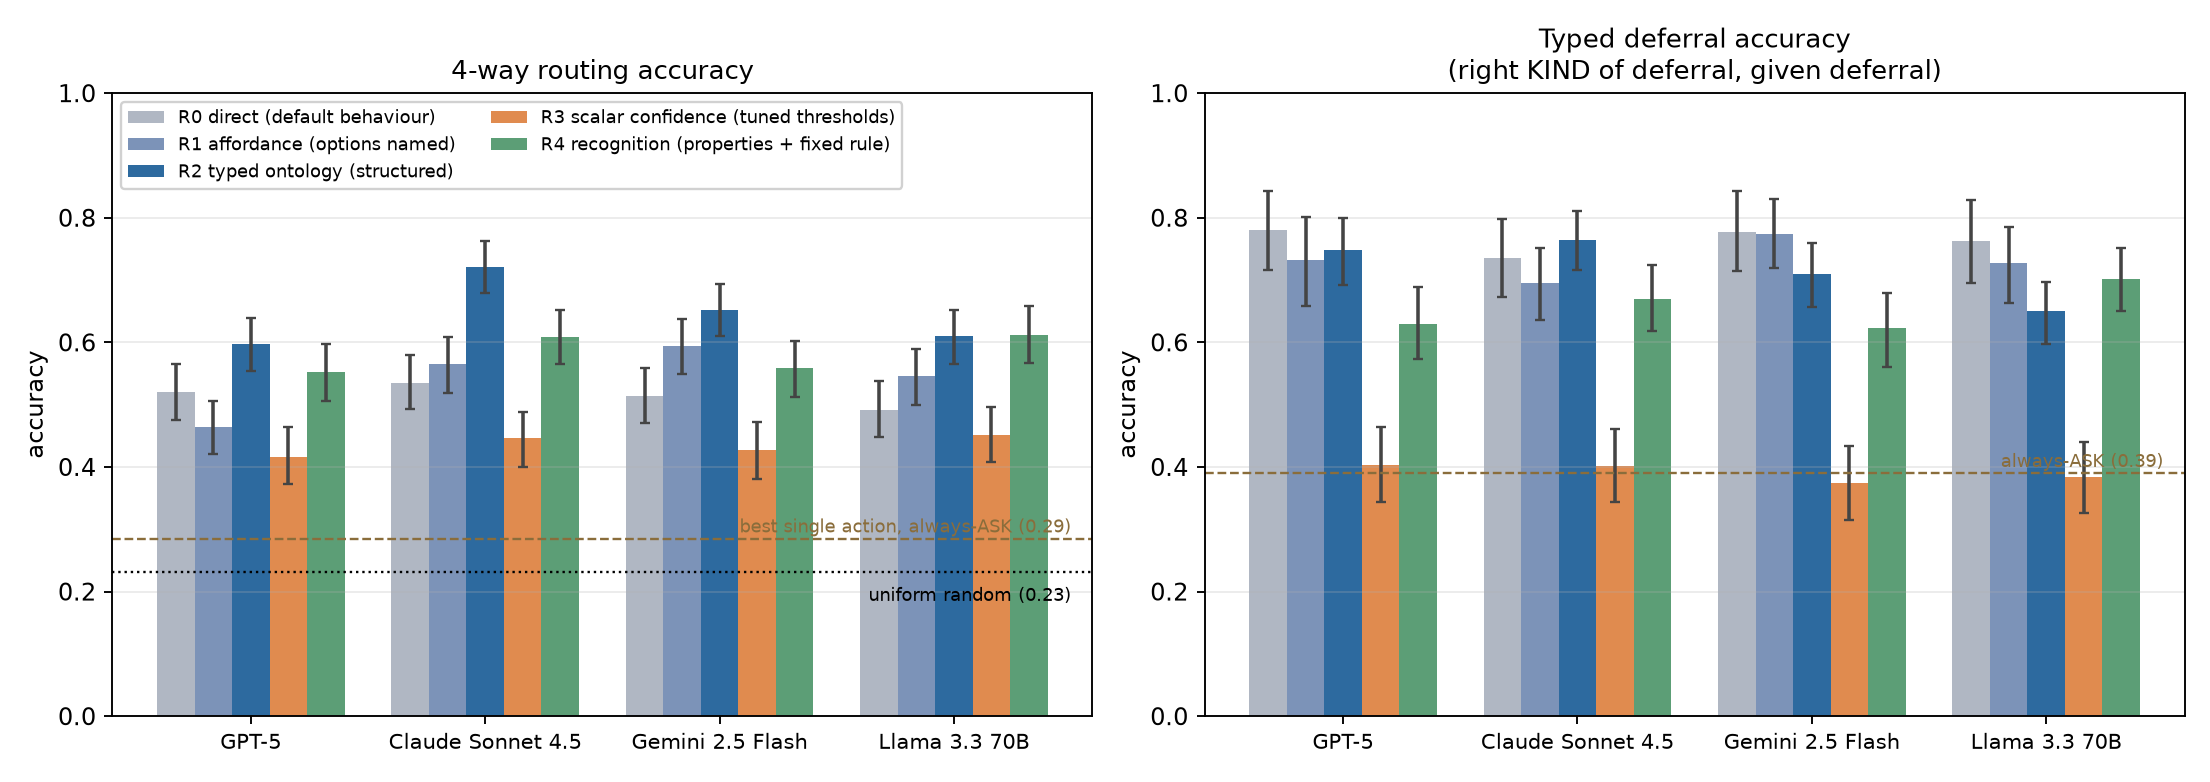
\includegraphics[width=0.95\linewidth]{figures/fig1_regime_accuracy.png}
    \caption{Four-way accuracy by elicitation regime on identical items ($n{=}480$), with
    bootstrap 95\% CIs. Typed prompting (\rtwo) is the top or joint-top regime for every model;
    routing a verbalised confidence (\rthree) is the worst for every model, despite being given the
    best cross-validated router that can be fitted to it. Dashed lines mark uniform random (0.231)
    and the best single-action policy (0.285).}
    \label{fig:regimeacc}
\end{figure}

\para{The head-to-head.} Typed prompting beats optimally-routed scalar confidence on every model,
by $+0.181$ (\gptfive), $+0.275$ (\claude), $+0.225$ (\gemini), and $+0.158$ (\llama) accuracy;
Cohen's $h = 0.36$, $0.57$, $0.46$, $0.32$; all $p_{\text{Holm}} < 10^{-8}$
(\figref{fig:regimeacc}, \tabref{tab:main}). Typed-deferral accuracy --- getting the right
\emph{kind} of withholding --- is 0.650--0.764 under typed prompting and 0.374--0.403 under the
scalar. This replicates \citet{unlu2026ssta} in direction at 15$\times$ the sample size and across
five models, and corrects the magnitude: their 91.7\% typed-deferral figure was an upper bound
produced by a single-context audit, and with contexts isolated we see 0.65--0.76.

\begin{table}[t]
    \centering
    \small
    \resizebox{\textwidth}{!}{%
    \begin{tabular}{@{}lccccc@{}}
        \toprule
        \multirow{2}{*}{\textbf{Model}} & \textbf{AUROC} & \textbf{Mean conf.} & \multicolumn{3}{c}{\textbf{AUROC, pairs of withholding types}} \\
        \cmidrule(lr){4-6}
         & \act \versus rest & \act/\ask/\refuse/\defer & \ask--\refuse & \ask--\defer & \defer--\refuse \\
        \midrule
        \gptfive & 0.814 & 83.3 / 50.8 / 23.6 / 11.0 & 0.721 & 0.780 & {\bf 0.507} \\
        \claude  & 0.824 & 82.7 / 45.2 / 18.9 / \phantom{0}6.8 & 0.669 & 0.741 & {\bf 0.436} \\
        \gemini  & 0.788 & 77.8 / 38.3 / \phantom{0}6.6 / 14.0 & 0.663 & 0.622 & {\bf 0.543} \\
        \llama   & 0.873 & 84.0 / 34.5 / \phantom{0}9.6 / 19.5 & 0.652 & 0.596 & {\bf 0.563} \\
        \bottomrule
    \end{tabular}%
    }
    \caption{Diagnostics for the verbalised-confidence regime (\rthree). The scalar carries real
    information about \emph{whether} to act (AUROC 0.79--0.87) and essentially none about
    \emph{which kind} of withholding is right: \defer \versus \refuse is at chance for every model and
    below chance for \claude (bold column). The mean-confidence column shows the models do not even
    order the two consistently --- \gptfive and \claude place \defer below \refuse, \gemini and
    \llama above it. Three deferral types cannot be recovered from an ordering of one number.}
    \label{tab:scalar}
\end{table}


\para{Why the scalar cannot work.} \Tabref{tab:scalar} gives the geometric reason. The confidence
number separates act from not-act well (AUROC 0.788--0.873) and is {\bf at chance at separating
\defer from \refuse} (0.436--0.563, below chance for \claude). Worse, the models do not order the
two consistently: \gptfive and \claude put \defer below \refuse in mean confidence, \gemini and
\llama above it. Three distinct reasons for not acting cannot be recovered from an ordering of one
number, and empirically they are not even consistently ordered.

\para{Is the scalar at least complementary?} No. A hybrid policy that uses the cross-validated
scalar for the \act gate --- its one strength --- and the typed judgment for the kind never beats
plain typed prompting, and for \claude it is significantly \emph{worse} (0.654 \versus 0.721,
$p_{\text{Holm}} = 1.1\times10^{-4}$). The same holds with a recognition-based second stage. The
scalar adds nothing the typed judgment does not already contain.

\para{Calibration and resolution.} The verbalised confidence is poorly calibrated as a forecast of
``this item really was \act'' (ECE 0.162--0.210 against a 0.27 base rate, mean stated confidence
0.364--0.446 --- systematically over-confident). It is also barely a scale: {\bf only 3--31\% of the
probability mass falls strictly between 0.05 and 0.95} (\gemini 3\%, \claude 17\%, \gptfive 18\%,
\llama 31\%). Asked for a number from 0 to 100, the models answer 0 or 100. Under an interaction
budget, ranking by $1-$confidence and asking on the least confident $b\%$ recovers roughly twice
random ask-recall (0.33--0.39 at $b = 20\%$ against 0.20 random) --- real but weak, and the typed
policies sit at similar recall with much better precision (\claude: ask-rate 0.24, recall 0.41,
precision 0.89).

\subsection{Experiment 3: stakes move the threshold, not the judgment}
\label{sec:e3}

Each of 240 items (60 per gold action) was shown under three announced-stakes frames prepended to
the system prompt, within-item. We exclude \gptfive: its stakes cells came back 68--100\% empty
when the API budget ran out, and missingness that asymmetric across the manipulated factor cannot
enter a factorial. The analysis pools \claude and \gemini.

\begin{figure}[t]
    \centering
    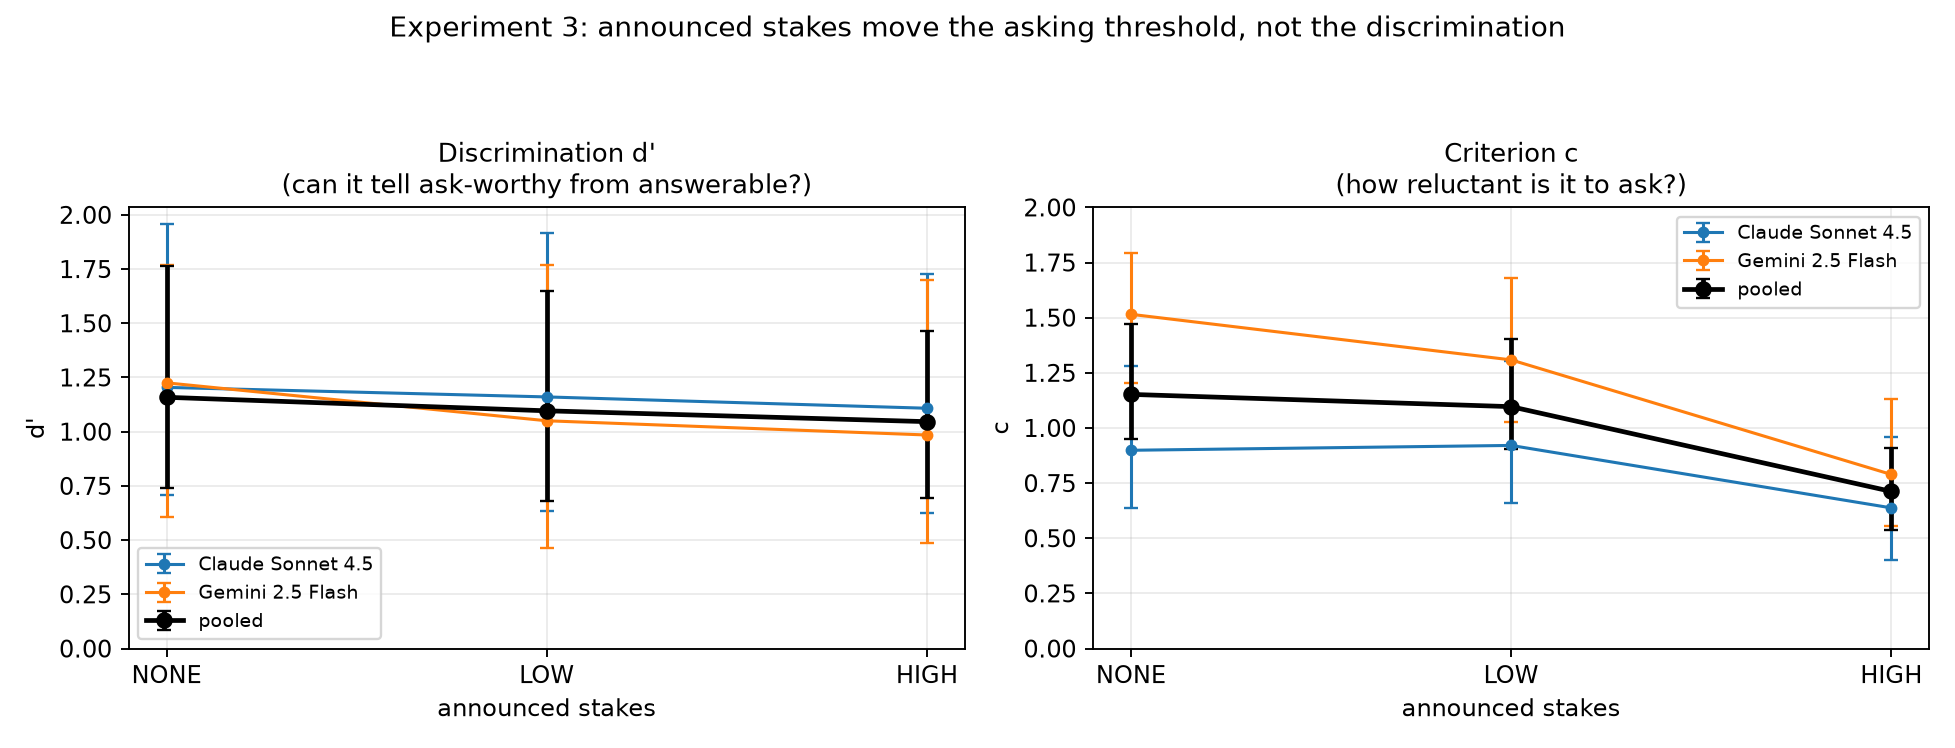
\includegraphics[width=0.95\linewidth]{figures/fig10_stakes_sdt.png}
    \caption{Announced stakes in signal-detection terms. Moving from \textsc{None} to \textsc{High}
    slides the criterion $c$ down decisively in both regimes while leaving $d'$ flat under the typed
    ontology and \emph{lowering} it under a plain ask-affordance. The manipulation buys
    indiscriminate caution, not calibrated caution.}
    \label{fig:sdt}
\end{figure}

\begin{table}[t]
    \centering
    \small
    \resizebox{\textwidth}{!}{%
    \begin{tabular}{@{}llcccc@{}}
        \toprule
        \textbf{Regime} & \textbf{Frame} & \textbf{Hit rate} & \textbf{False alarm} & \textbf{$d'$ [95\% CI]} & \textbf{Criterion $c$ [95\% CI]} \\
         & & (ask $\mid$ gold \ask) & (ask $\mid$ gold \act) & & \\
        \midrule
        \multirow{3}{*}{\rtwo (typed)}
          & \textsc{None} & 0.283 & 0.042 & 1.159 [0.74, 1.77] & 1.152 [0.95, 1.47] \\
          & \textsc{Low}  & 0.292 & 0.050 & 1.096 [0.68, 1.65] & 1.097 [0.90, 1.40] \\
          & \textsc{High} & 0.425 & 0.108 & 1.046 [0.70, 1.46] & {\bf 0.712} [0.54, 0.91] \\
        \midrule
        \multirow{3}{*}{\rone (free text)}
          & \textsc{None} & 0.333 & 0.042 & 1.301 [0.91, 1.94] & 1.081 [0.88, 1.42] \\
          & \textsc{Low}  & 0.350 & 0.058 & 1.184 [0.81, 1.70] & 0.977 [0.79, 1.26] \\
          & \textsc{High} & 0.558 & 0.283 & {\bf 0.720} [0.41, 1.06] & {\bf 0.213} [0.06, 0.39] \\
        \midrule
        \multicolumn{6}{@{}l@{}}{\emph{Paired bootstrap of the change, \textsc{High} $-$ \textsc{None} (4{,}000 resamples over items)}} \\
        \rtwo (typed)     & & \multicolumn{2}{l}{$\Delta d' = -0.112$ [$-0.623$, $+0.225$], $p = 0.53$} & \multicolumn{2}{l}{$\Delta c = -0.440$ [$-0.687$, $-0.274$], $p < 0.001$} \\
        \rone (free text) & & \multicolumn{2}{l}{$\Delta d' = -0.581$ [$-1.205$, $-0.109$], $p = 0.013$} & \multicolumn{2}{l}{$\Delta c = -0.868$ [$-1.202$, $-0.651$], $p < 0.001$} \\
        \bottomrule
    \end{tabular}%
    }
    \caption{Announced stakes, decomposed by signal detection theory over 240 items shown under
    three frames within-item, pooled over \claude and \gemini. Announcing high stakes moves the
    \emph{criterion} decisively in both regimes and leaves \emph{discrimination} statistically
    unchanged under the typed ontology --- and makes it significantly worse under a plain
    ask-affordance, where the false-alarm rate rises almost sevenfold. Telling a model the stakes
    are high makes it more anxious, not a better judge.}
    \label{tab:stakes}
\end{table}


\para{The manipulation works, in the wrong way.} Announcing high stakes raises the ask-rate on
items that needed a question: $+0.133$ typed ($p_{\text{Holm}} = 0.005$) and $+0.208$ free-text
($p_{\text{Holm}} = 1.4\times10^{-4}$), both paired \textsc{High} \versus \textsc{Low}. But it raises
the false-alarm rate on genuinely answerable items as much or more (0.042 $\rightarrow$ 0.108 typed,
0.042 $\rightarrow$ 0.283 free-text). A paired bootstrap of the \emph{change} between frames
(\tabref{tab:stakes}, \figref{fig:sdt}) gives $\Delta c = -0.440$ [$-0.687$, $-0.274$], $p<0.001$
with $\Delta d' = -0.112$ [$-0.623$, $+0.225$], $p = 0.53$ under the typed ontology. Under a plain
ask-affordance --- which is what a deployed assistant actually has --- discrimination gets
{\bf significantly worse}: $\Delta d' = -0.581$ [$-1.205$, $-0.109$], $p = 0.013$.

\para{Additive, not interactive.} An item-clustered logistic regression of $P(\ask)$ on ambiguity
and announced stakes says the same thing in one number: \texttt{ambiguous} $\beta = +2.553$
($p = 4.3\times10^{-9}$) and \texttt{high} $\beta = +0.630$ ($p = 0.009$) are both large, and the
interaction \texttt{ambiguous $\times$ high} is $\beta = {\bf +0.010}$, $p = 0.97$. A model that used
stakes properly would show a positive interaction --- asking \emph{more where it matters}, not
everywhere.

\para{The cost is concrete.} Under \textsc{High}, the act-rate on genuinely answerable requests
falls from 0.842 to 0.708 (typed) and from 0.925 to 0.550 (free text). Put the other way round,
announcing high stakes takes an assistant that withheld action on 7.5\% of answerable requests and
turns it into one that withholds on {\bf 45\%} of them.

\para{Item-level stakes, where nobody tells the model anything.} Among \inthree items whose gold
action is \ask, the ask-rate rises with the annotated importance of the missing detail: 0.045 at
importance 2 \versus 0.306 at importance 3 under typed prompting (item-level Mann--Whitney $p = 0.006$,
$n = 22$ \versus $9$). This is the one place where behaviour tracks stakes without being told. It is
also confounded --- a more important missing detail is plausibly also a more obvious one --- so we
treat it as suggestive rather than as evidence for the stakes clause.

\subsection{Experiment 4: training helps in-distribution, and the signal was already there}
\label{sec:e4}

\begin{figure}[t]
    \centering
    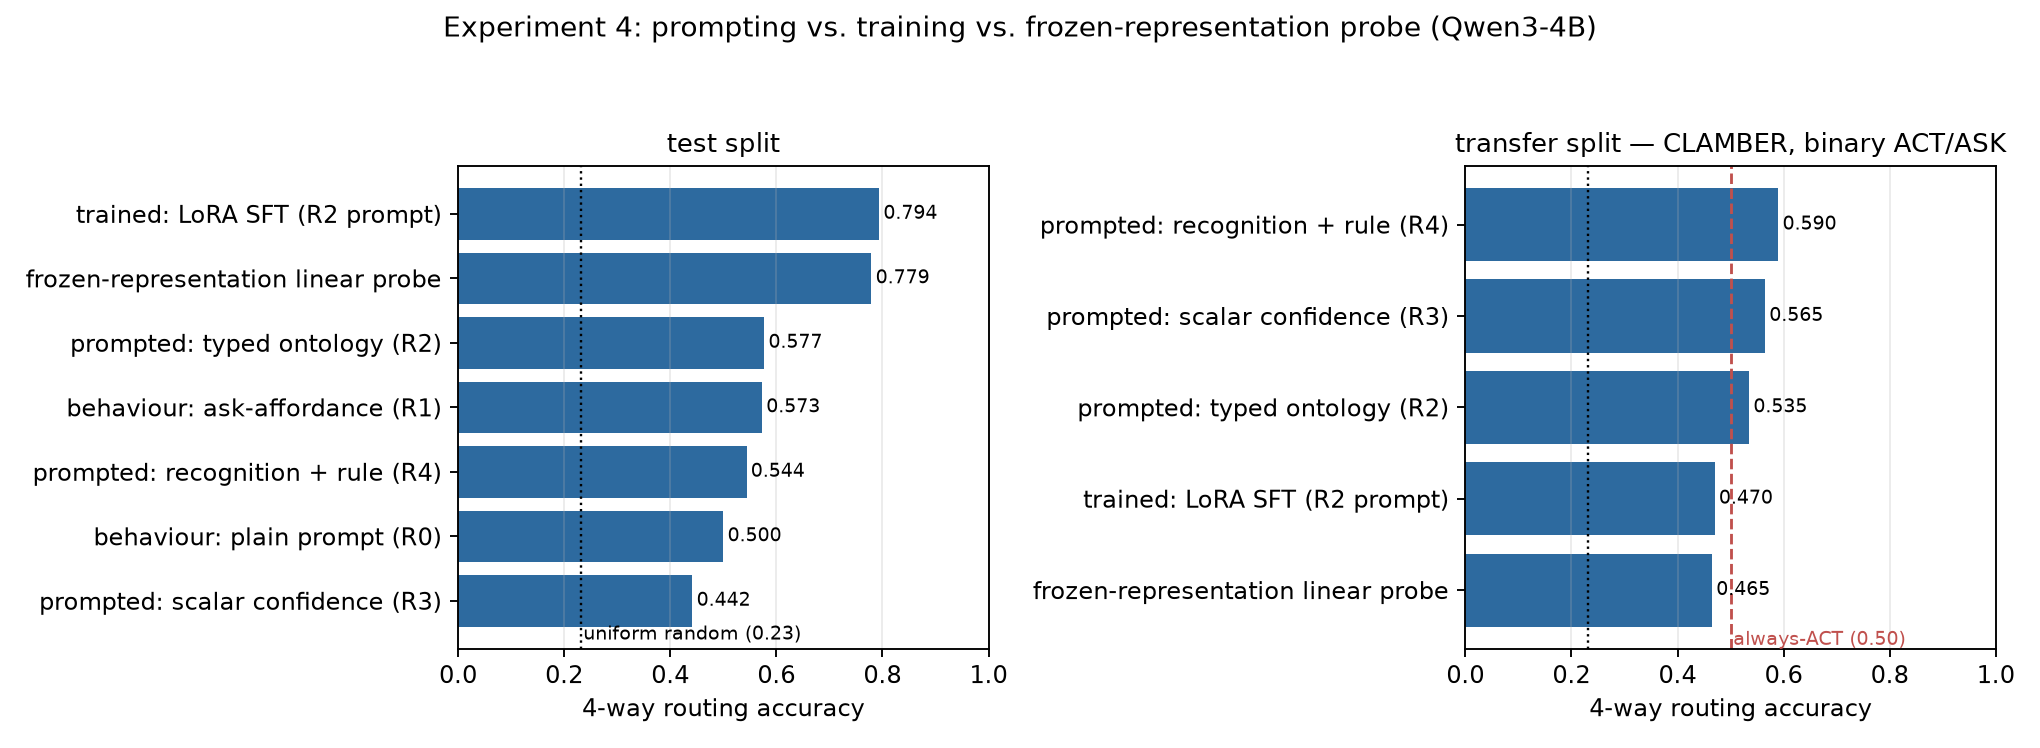
\includegraphics[width=0.95\linewidth]{figures/fig7_local_training.png}
    \caption{Prompting, training, and probing on \qwen. LoRA SFT reaches 0.794 and cuts
    over-commitment to 1.4\%, but a frozen linear probe on the \emph{base} model's hidden state at
    the final prompt token gets within 1.5 points of it with no training at all --- 20 points above
    what the same model does when simply asked. On the out-of-source transfer split both supervised
    conditions fall below the untrained prompted baselines.}
    \label{fig:local}
\end{figure}

\begin{table}[t]
    \centering
    \small
    \resizebox{\textwidth}{!}{%
    \begin{tabular}{@{}lccccc@{}}
        \toprule
        \textbf{Condition} & \textbf{Test acc [95\% CI]} & \textbf{Macro-F1} & \textbf{ASK-F1} & \textbf{Over-commit $\downarrow$} & \textbf{Transfer acc} \\
        \midrule
        \multicolumn{6}{@{}l@{}}{\emph{Behaviour}} \\
        plain prompt (\rzero)          & 0.500 [0.456, 0.546] & 0.481 & 0.200 & 0.581 & --- \\
        ask-affordance (\rone)         & 0.573 [0.529, 0.617] & 0.568 & 0.383 & 0.413 & --- \\
        \midrule
        \multicolumn{6}{@{}l@{}}{\emph{Prompted}} \\
        typed ontology (\rtwo)         & 0.577 [0.533, 0.621] & 0.577 & 0.489 & 0.168 & 0.535 \\
        scalar confidence (\rthree)    & 0.442 [0.398, 0.483] & 0.358 & 0.310 & 0.171 & 0.565 \\
        recognition $+$ rule (\rfour)  & 0.544 [0.500, 0.590] & 0.539 & 0.530 & 0.131 & {\bf 0.590} \\
        \midrule
        \multicolumn{6}{@{}l@{}}{\emph{Supervised}} \\
        LoRA SFT on typed routing      & {\bf 0.794} [0.756, 0.829] & {\bf 0.790} & {\bf 0.798} & 0.014 & 0.470 \\
        frozen linear probe (base model) & 0.779 [0.744, 0.817] & 0.773 & 0.766 & {\bf 0.009} & 0.465 \\
        \bottomrule
    \end{tabular}%
    }
    \caption{Prompting, training, and probing on one open-weight model (\qwen). The open model
    reproduces both frontier patterns on its own: typed prompting beats scalar routing by 13.5
    points on identical items, and a plain prompt over-commits on 58\% of items that should have
    been withheld. LoRA SFT reaches {\bf 0.794} in-distribution (+0.217 over the same model with
    the same ontology, McNemar $p = 8.0 \times 10^{-15}$), but a frozen linear probe on the
    \emph{untrained} model's hidden state already reaches 0.779 --- the routing signal was in the
    representation, and training mostly added a read-out. Neither survives a change of source: on
    the transfer split both fall below the untrained prompted baselines, and every condition sits
    within $\pm 0.09$ of the always-\act policy at 0.50.}
    \label{tab:local}
\end{table}


\para{The frontier patterns reproduce on an open model.} \qwen shows both effects on its own
(\tabref{tab:local}): typed prompting (0.577) beats scalar routing (0.442) by 13.5 points on
identical items, the same direction and roughly the same size as the four frontier models, and
under a plain prompt it acts on {\bf 58\%} of items it should have withheld action on, which the
typed prompt cuts to 17\% and the recognition rule to 13\%. Whatever this is, it is not an artefact
of one lab's post-training.

\para{Training works, in-distribution.} LoRA SFT on 2{,}576 prompt$\rightarrow$action pairs reaches
{\bf 0.794}, $+0.217$ over the same model prompted with the same ontology (McNemar
$p = 8.0\times10^{-15}$, $b{=}145$ / $c{=}41$), with over-commitment down to 0.014 and ASK-F1 up
from 0.489 to 0.798 --- in under two hours on one shared A6000.

\para{But the signal was already in the representation.} A logistic regression on the last hidden
state at the final prompt token of the \emph{base} model --- no fine-tuning, no generation ---
reaches 0.779, {\bf 20 points above what the same model does when asked} (McNemar
$p = 6.3\times10^{-12}$), within 1.5 points of the fine-tuned model. Read together with the SFT
result: LoRA training did not teach the model to route, it taught it to \emph{read out} a routing
signal its frozen representation already carried. That is the representation-level version of the
recognition--behaviour gap in \secref{sec:e1}.

\para{Neither transfers.} On the out-of-source split the SFT model drops to 0.470 and the probe to
0.465 --- both \emph{below} the untrained prompted baselines (0.535--0.590), with the differences
not significant in either direction (McNemar $p = 0.11$ and $0.13$). The blunter framing is worse:
\clamber is binary, so the relevant reference is always-\act at 0.50, and every condition ---
trained, probed, or prompted --- sits within $\pm 0.09$ of just answering everything. The TF-IDF
control shows the same shape (0.702 in-source $\rightarrow$ 0.355 out-of-source). Nothing in this
study demonstrates a routing policy that generalises across sources.

\subsection{Where the errors go}
\label{sec:errors}

\begin{figure}[t]
    \centering
    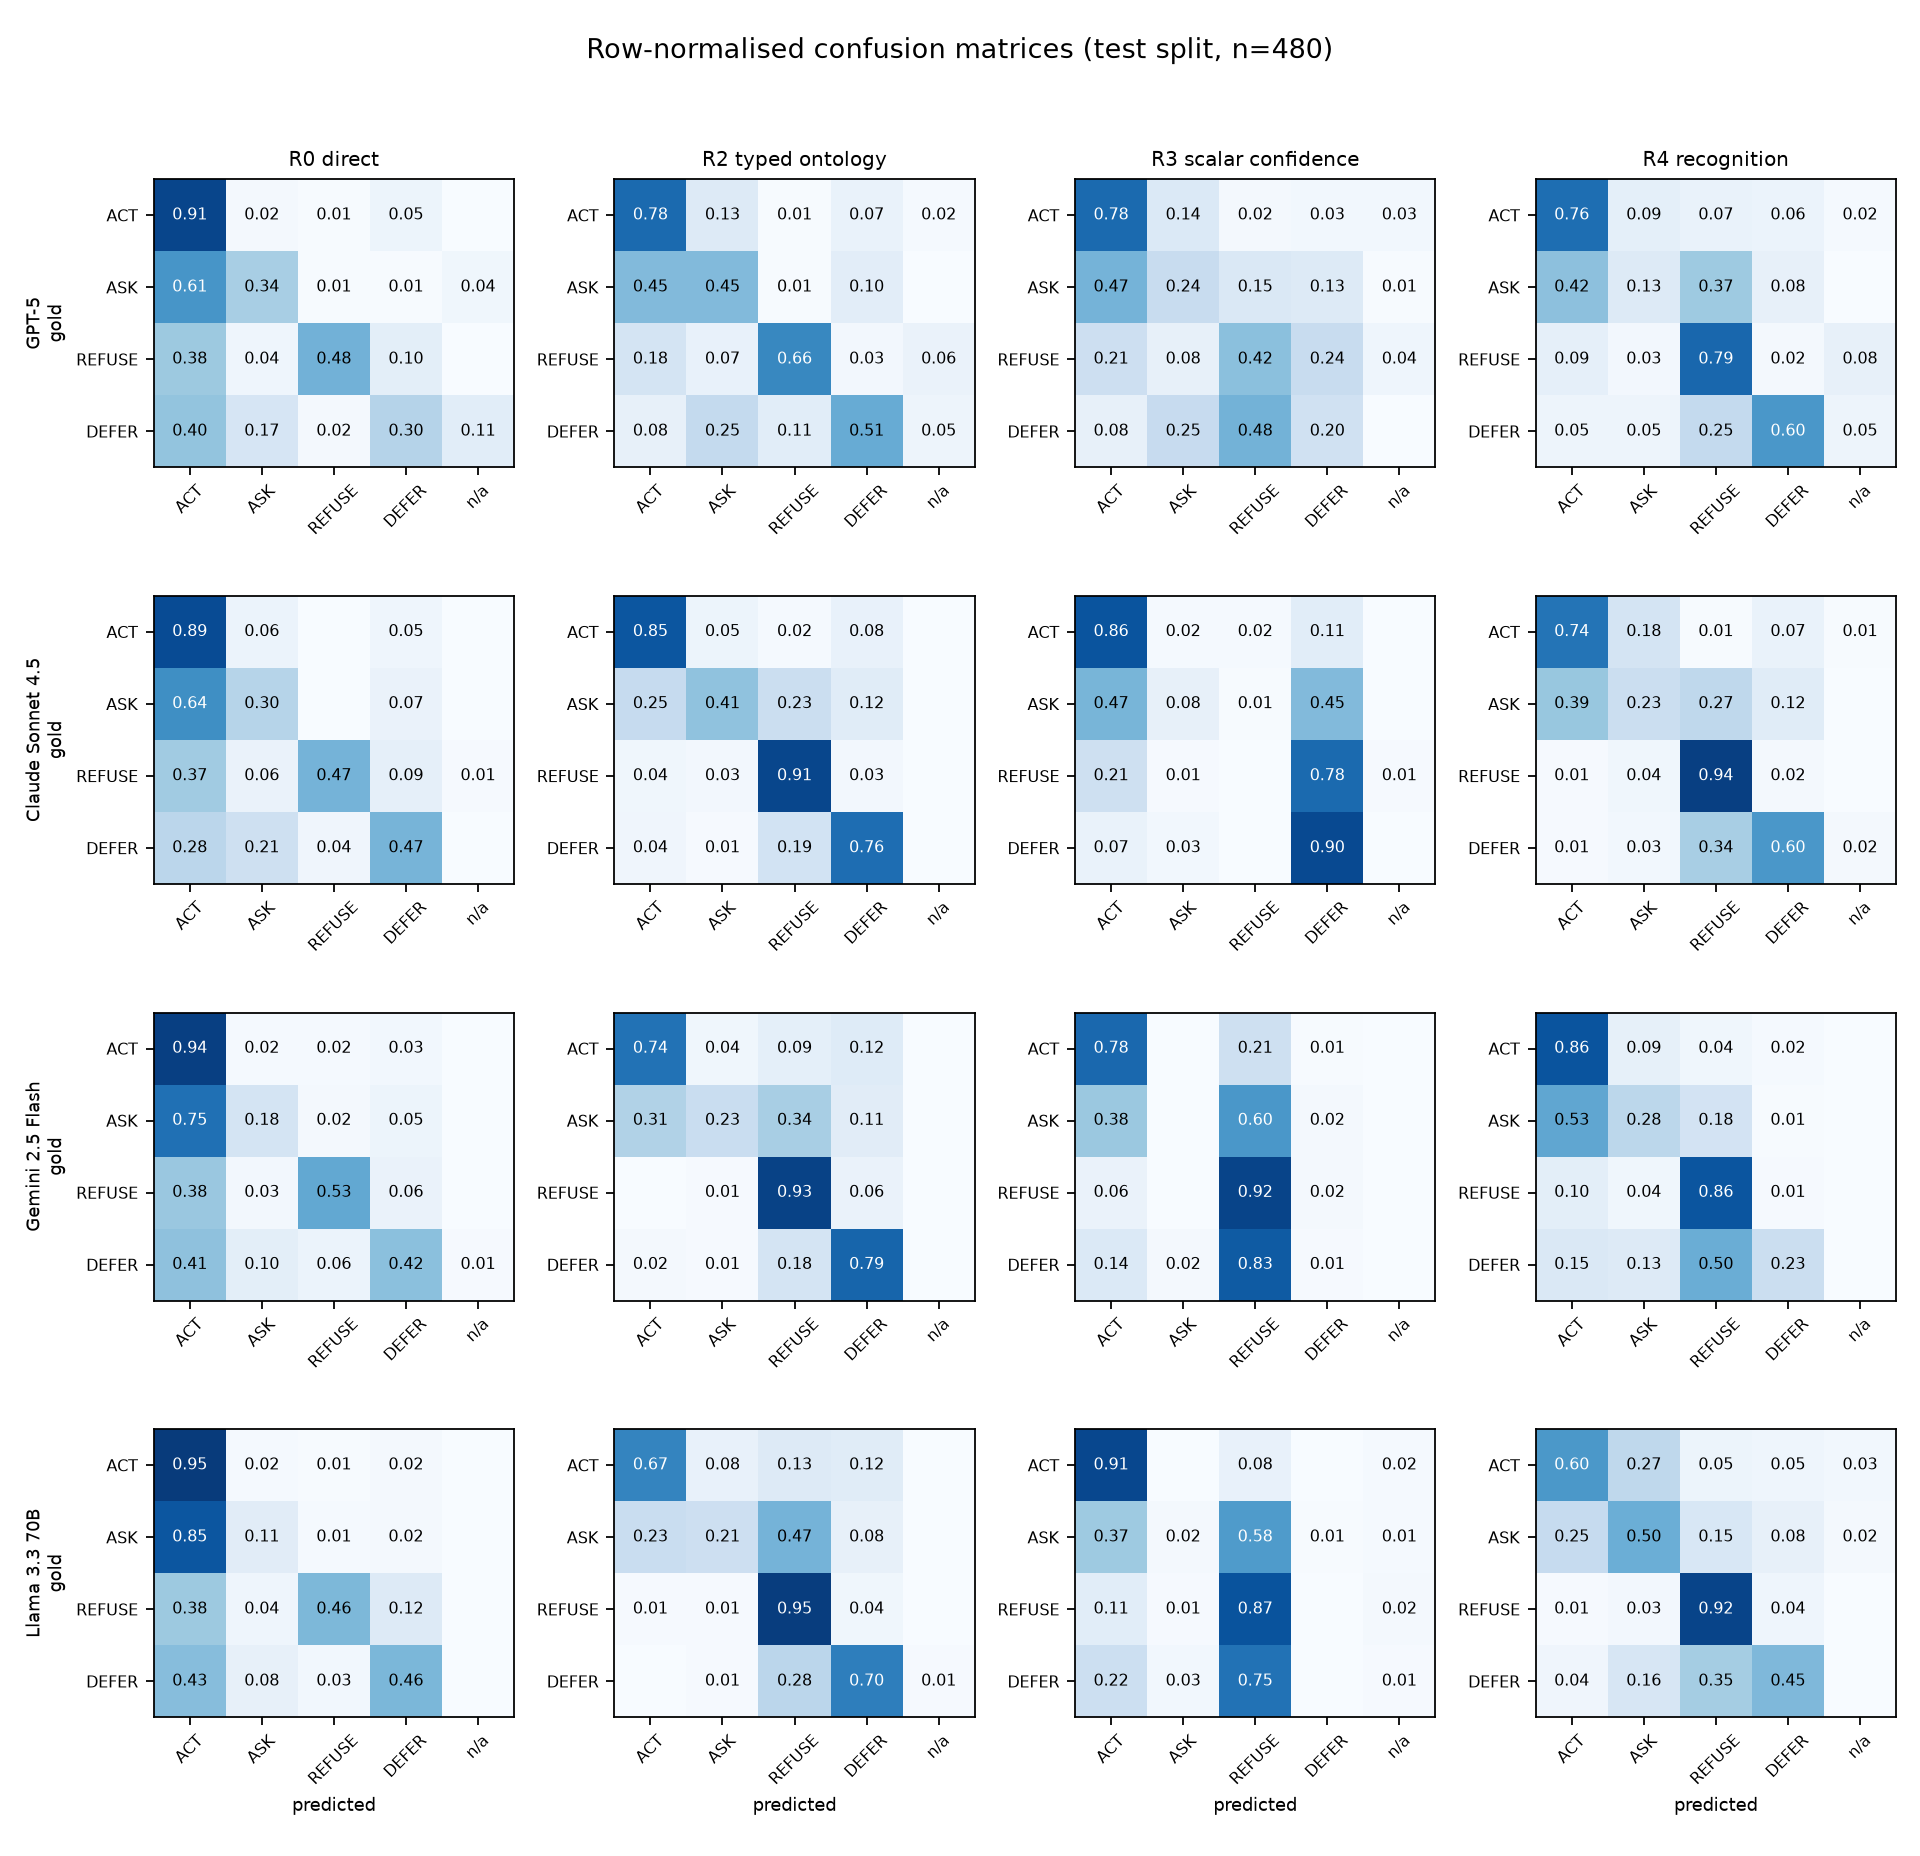
\includegraphics[width=0.95\linewidth]{figures/fig3_confusion_matrices.png}
    \caption{Confusion matrices by regime (rows = gold, columns = predicted). Two structures are
    visible. Under a plain prompt the mass sits in the \ask $\rightarrow$ \act cell: models answer
    under-specified requests. Under the scalar router the mass collapses into a single
    low-confidence label --- \defer for \claude, \refuse for \gemini and \llama --- so the router is
    making a two-way choice and labelling it three ways.}
    \label{fig:confusion}
\end{figure}

Pooling over the four models, four patterns stand out.

\para{The dominant default error is answering an under-specified request.} Under a plain prompt,
390 of 548 \ask items ({\bf 71\%}) are answered outright. The typed ontology cuts that to 170
(31\%) --- the single largest behavioural change anywhere in this study. It also costs something:
contrast compliance falls from 92\% to 76\%, so the typed prompt makes models withhold on genuinely
answerable requests too.

\para{Clarify-versus-abstain is exactly the confusion \citet{baan2026bag} named.} Under typed
prompting, 144 of 548 \ask items are routed to \refuse --- 26\%, almost as many as are routed
correctly (178). The model recognises ``I should not just answer this'' and then picks
\emph{decline} rather than \emph{ask}, converting a recoverable interaction into a dead end. No
scalar-confidence route touches this, because the scalar cannot tell \refuse from \defer, let alone
\ask from \refuse.

\para{The scalar router collapses two categories into one, visibly.} \Figref{fig:confusion} shows
what collapse means concretely: the cross-validated router assigns its lowest-confidence bin to a
single label and everything low-confidence lands there. For \claude that bin is \defer (\defer
recall 0.90, but 78\% of \refuse items sent to \defer); for \gemini and \llama it is \refuse
(\refuse recall 0.92/0.87, but 83\%/75\% of \defer items sent to \refuse).

\para{\defer is systematically misread as \refuse} (77/408, 19\%, under typed prompting), matching
the property result that models judge their own capability blocks to be indeterminacies of the
world. Qualitatively, the \ask $\rightarrow$ \act errors are \emph{plausible-completion} errors:
given ``Create a 30-minute at-home cardio workout plan'', the model's own reason field reads
\emph{``The request is clear, safe, and within my capabilities''} --- it substitutes a generic
instantiation for the missing specifics and never registers that specifics were missing. The
\defer $\rightarrow$ \refuse errors are attribution errors: for ``a line-by-line analysis of every
piece of legislation passed since 1789'' the reason reads \emph{``This request has no determinate
scope''} rather than ``this exceeds what I can produce''.

\subsection{Is any of this worth deploying?}
\label{sec:utility}

Accuracy prices every error the same, and the hypothesis is explicitly about stakes. We therefore
score every policy under a cost model with one free parameter $K$, the cost of acting on a request
that should have been withheld (correct action $+1$, needless question $-0.3$, needless refusal
$-1.0$, withheld for the wrong reason $+0.2$).

\begin{table}[t]
    \centering
    \small
    \begin{tabular}{@{}lccccc@{}}
        \toprule
        \textbf{Policy} & $K{=}1$ & $K{=}3$ & $K{=}5$ & $K{=}10$ & $K{=}30$ \\
        \midrule
        oracle                        & $+1.00$ & $+1.00$ & $+1.00$ & $+1.00$ & $+1.00$ \\
        always \ask                   & $+0.29$ & $+0.29$ & $+0.29$ & $+0.29$ & $+0.29$ \\
        always \act (today's default) & $-0.46$ & $-1.93$ & $-3.39$ & $-7.04$ & $-21.67$ \\
        \midrule
        \claude, typed   & {\bf +0.63} & {\bf +0.46} & {\bf +0.28} & $-0.15$ & $-1.90$ \\
        \llama, typed    & $+0.51$ & $+0.37$ & $+0.23$ & $-0.12$ & $-1.54$ \\
        \gemini, typed   & $+0.53$ & $+0.35$ & $+0.16$ & $-0.31$ & $-2.18$ \\
        \gptfive, typed  & $+0.39$ & $-0.03$ & $-0.46$ & $-1.51$ & $-5.72$ \\
        \claude, default behaviour  & $+0.21$ & $-0.45$ & $-1.11$ & $-2.75$ & $-9.34$ \\
        \gptfive, default behaviour & $+0.14$ & $-0.62$ & $-1.38$ & $-3.27$ & $-10.86$ \\
        \midrule
        \qwen frozen probe & {\bf +0.69} & {\bf +0.68} & {\bf +0.67} & {\bf +0.64} & {\bf +0.51} \\
        \qwen LoRA SFT     & $+0.70$ & $+0.68$ & $+0.66$ & $+0.61$ & $+0.40$ \\
        \bottomrule
    \end{tabular}
    \caption{Mean utility per request when errors are priced. $K$ is the cost of acting on a
    request that should have been withheld; a correct action scores $+1$, a needless question
    $-0.3$, a needless refusal $-1.0$, and withholding for the wrong reason $+0.2$. Read down the
    columns: every frontier model's best prompted policy crosses below the trivial
    \emph{always-\ask} policy at $K \approx 5$--$10$ and goes negative shortly after, and every
    model's \emph{default behaviour} goes negative between $K=1$ and $K=2$. The two supervised
    \qwen policies stay above always-\ask across the whole sweep --- but \tabref{tab:local} shows
    neither survives a change of source, so that is a statement about \carb, not about deployment.}
    \label{tab:utility}
\end{table}


\begin{figure}[t]
    \centering
    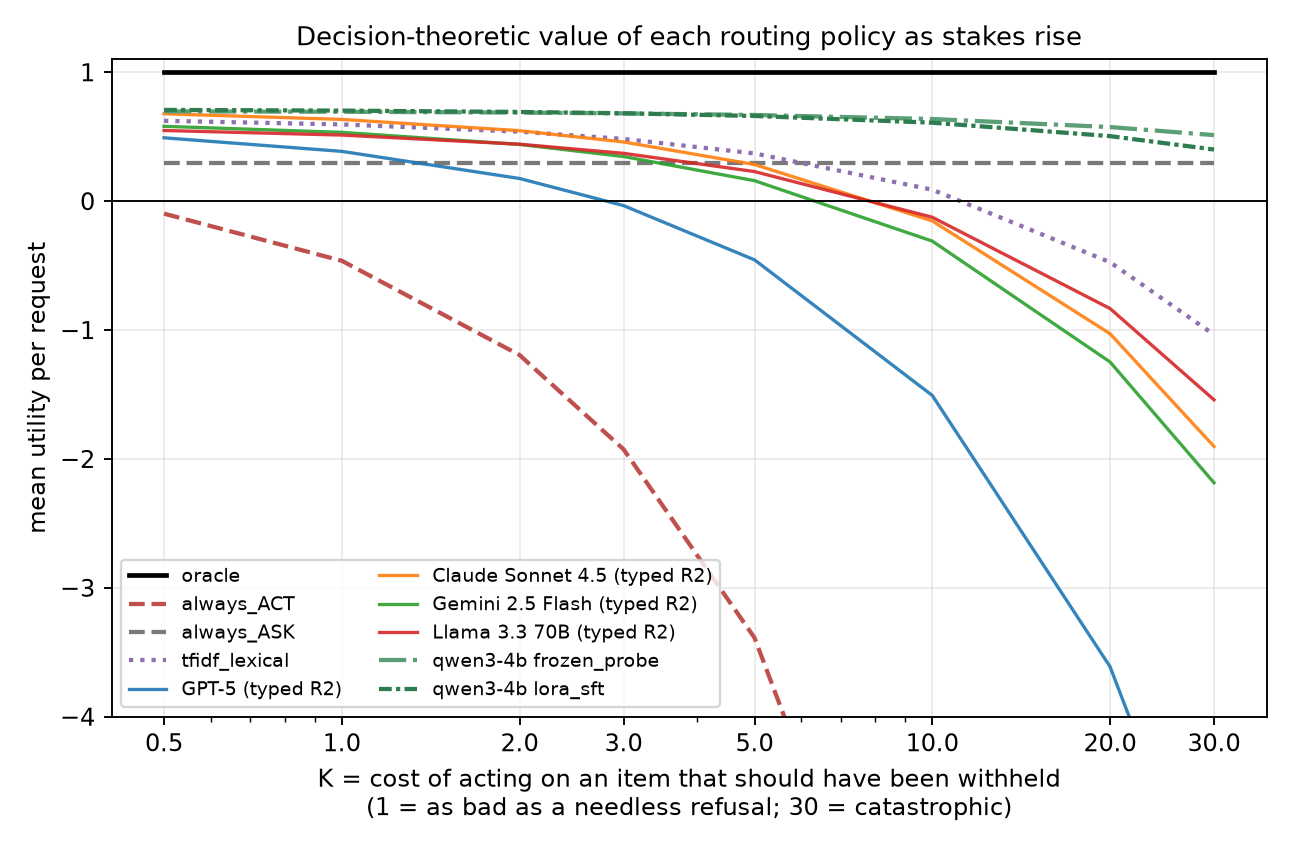
\includegraphics[width=0.95\linewidth]{figures/fig8_utility_vs_stakes.png}
    \caption{Mean utility per request as the cost $K$ of an unwarranted action rises. The flat
    always-\ask line is the bar that matters: every frontier model's best prompted policy crosses
    below it at $K \approx 5$--$10$. $K = 10$ is not extreme --- it is ``a wrong action costs ten
    times a needless refusal'', about 33$\times$ a needless clarifying question, which is mild for
    anything that writes to a database, sends a message, or gives medical advice.}
    \label{fig:utility}
\end{figure}

\Tabref{tab:utility} and \figref{fig:utility} give the deployment-relevant reading. Every model's
\emph{default behaviour} goes negative between $K=1$ and $K=2$, \ie as soon as a wrong action costs
even slightly more than a needless refusal. Every frontier model's best prompted policy crosses
below the trivial always-\ask policy at $K \approx 5$--$10$ and goes negative shortly after. Only
the two in-distribution supervised \qwen policies stay above always-\ask across the sweep, and
\secref{sec:e4} has already shown neither survives a change of source. The conclusion is not that
these models cannot route; it is that {\bf their routing is not yet good enough to beat asking
every time} in exactly the regime the hypothesis cares about.

\subsection{Sensitivity to the label mapping}
\label{sec:sensitivity}

Because the gold labels are inherited rather than authored, the mapping table is the main place a
systematic error could enter. We recomputed every model $\times$ regime cell three ways: dropping
the two contested mapping cells, under an alternative mapping that sends false-presupposition items
to \refuse, and under a capability re-audit of the \inthree items. Individual accuracies move by at
most {\bf 0.068}, and {\bf both headline orderings survive in all 16 model $\times$ variant cells}:
typed beats scalar everywhere, and recognition beats default behaviour everywhere. The rank order
is not completely invariant --- for \llama the pre-registered labels put recognition 0.003 above
typed, which every variant reverses --- but no conclusion above depends on that pair.
